%% \columnbreak
%% \section*{\LARGE Modelling synaptic lifetime distributions with Kesten processes}

\section{Introduction}

The wiring of cortical circuits is highly dynamic. Spine sizes fluctuate even in the absence of neural activity and there is constant synaptic turnover \cite{Loewenstein2015}. In models of cortical circuits, two major mechanisms are typically considered to drive the efficacies of synaptic connections: Spike-timing dependent plasticity (STDP) is often assumed to strengthen or weaken synaptic connections in an additive manner, independent of the current weight. Synaptic normalization, on the other hand, acts multiplicatively on synapses by scaling their efficacies by a varying factor that depends on the availability of synaptic resources \cite{Triesch2017} (see Fig.~\ref{fig:spines}).



\begin{center}\vspace{0.5cm}
  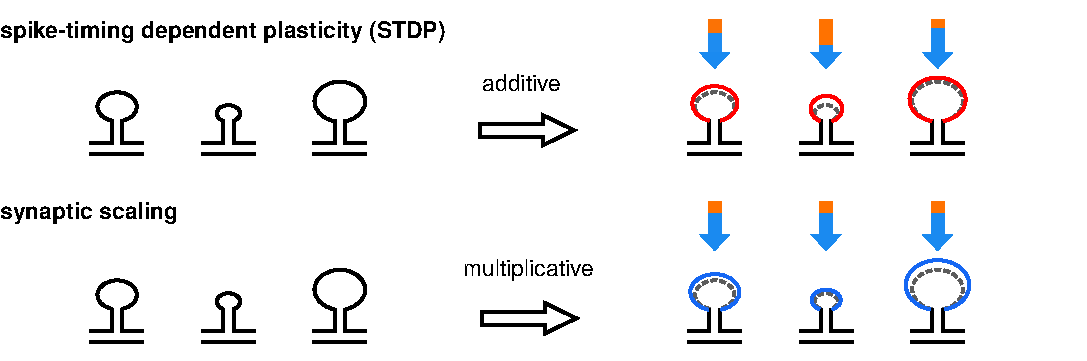
\includegraphics[width=\columnwidth]{%
    /home/fh/pub/graphics/synapse_size_dynamics/synapse_size_dynamics.png} %
  \captionof{figure}{Adapted Kesten simulation model allows the tracking of lifetimes and size distributions}
  \label{fig:spines}
\end{center}\vspace{2cm}


To model the fluctuations of synaptic spine sizes over time, a stochastic process called Kesten process has been suggested \cite{Kesten1973, Statman2014}. In this process, a random variable $X_n$ at time step $n$ is updated by scaling it with a random multiplicative factor $a_n$ and then adding a random increment $b_n$ according to
%
\begin{align}
  X_{n+1} = a_n X_n + b_n. \label{eq:kesten}
\end{align}
%
This stochastic model has been successfully used to describe the distribution of synaptic spine sizes measured in experiments. Here we extend the Kesten process by including the explicit creation and elimination of spines. Simulation and analysis of the model reveals that the distribution of lifetimes approximately follow a power law, as has been recently identified in experiments in the rat neocortex \cite{Loewenstein2015}.


%% In an experimental study by \textcite{Loewenstein2015} chronic in-vivo two-photon imaging suggested that the lifetime dynamics of spines in the neocortex follow a power law. Motivated by results from detailed network simulations, we here consider a simple stochastic model based on the Kesten process in order to analyze how different properties of a cortical network might affect the lifetime distributions of synaptic spines.

\vspace{-0.4cm}
\section*{Model}

Kesten processes have been used before \cite{Statman2014} to describe spine size dynamics. In this model, a given spine size $X_n$ at time step $n$ is updated as
%
\begin{align}
  X_{n+1} = a_n X_n + b_n. \label{eq:kesten}
\end{align}
%
In this further simplified form we take $a_n$ to be a fixed value of $a_n < 1$, while the additive change is in each time step drawn from a normal distribution, $b_n \sim \mathcal{N}(\mu_b, \sigma_b^2)$. Then, to model synapse growth and pruning processes, we consider a population of $N$ synapses. Each synapse has a random time $T_{\mathrm{init}}$, uniformly distributed in $[0,T_{\text{max}}]$, at which it is initialized with size $X_0$. The synapse size $X_t$ then evolves according to \eqref{eq:kesten}.

\medskip

The lifetime of the synapse is the number of time steps from $T_{\text{init}}$ until for the first time $X_t < X_{\mathrm{prune}}$. In this case the synapse gets pruned and a new synapse with size $X_0$ is inserted in the network (Fig.~\ref{fig:km}). In the case that $X_t$ doesn't fall below $X_{\mathrm{prune}}$ until $T_{\text{max}}$, the lifetime is recorded as $T=T_{\text{max}}-T_{\text{init}}$. At the end of the simulation the sizes $X_{T_{\text{max}}}$ are recorded for all $N$ synapses.

\begin{center}\vspace{1cm}
  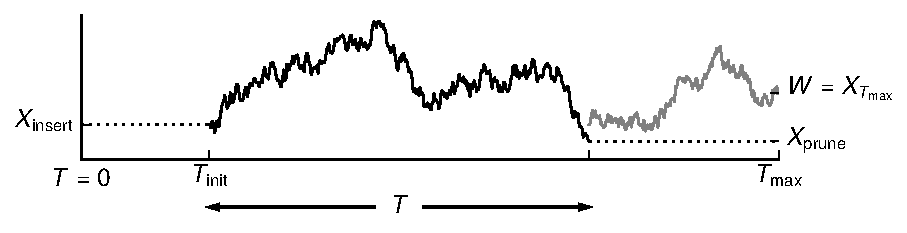
\includegraphics[width=0.85\columnwidth]{%
    figures/abstract_fig.pdf}
  %% /home/fh/sci/lab/syn_lt/kesten_model/note_x/km_ca_rts_dd/img/abstract_fig.png}
  \captionof{figure}{Adapted Kesten simulation model allows the tracking of lifetimes and size distributions}
  \label{fig:km}
\end{center}\vspace{1.4cm}


\section*{Results}

We simulated \SI{5e5} synapses evolving as Kesten processes and recorded lifetime and weight distributions. For unbiased additive change ($\mu_b =0$), a power law like distribution of synaptic lifetimes emerges (Fig.~\ref{fig:lifetimes}A). The distribution of spine sizes $X_{T_{\text{max}}}$ resembles a log-normal distribution, as one might expect from findings on the synaptic weight distributions in cortical circuits \cite{Song2005}.

\vspace{1.2cm}
\begin{overpic}[width=\columnwidth]%
  % 110, 133
  {figures/lifetimes_weights.pdf}
  %\put(32,\ylin){anisotropic}
  \put(1,28){\normalfont \textbf{A}}
  \put(52,28){\normalfont \textbf{B}}
\end{overpic}
\captionof{figure}[format=hang,indention=1cm]{Dynamical properties of network connectivity modelled by Kesten processes. \textbf{A} Lifetime distribution of synapses created at time step $T_{\text{init}}$ uniformly distributed in $[0, T_{\text{max}}]$. \textbf{B} Distribution of spine sizes $X_{T_{\text{max}}}$ at time step $X_{T_{\text{max}}}$ (grey) and log-normal fit (red). Parameters for both: $a=0.9987$, $\mu_b=0$, $\sigma_b^2=0.22$, $X_{\text{insert}}=0.1$, $X_{\text{prune}}=0.01$. \label{fig:lifetimes}}

\vspace{3cm}

%% \begin{center}\vspace{1cm}
%%   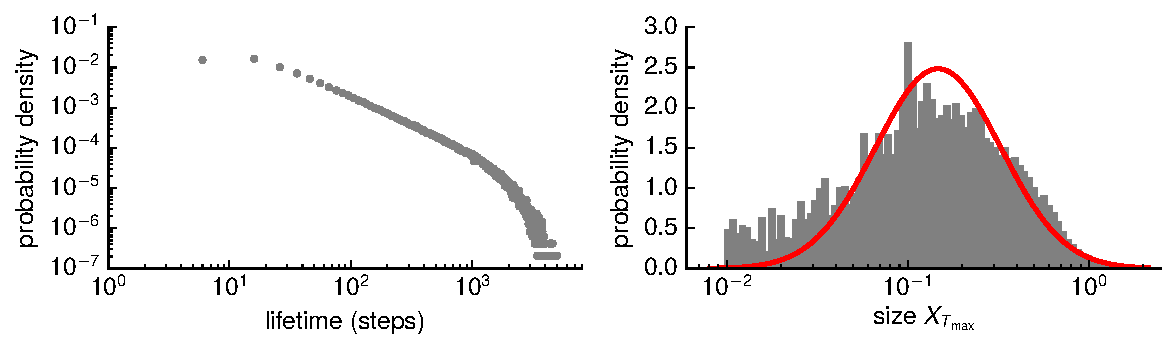
\includegraphics[width=\columnwidth]{%
%%     %% /home/fh/sci/lab/syn_lt/kesten_model/note_x/km_ca_rts_dd/img/lifetimes_weights.png}
%%     figures/lifetimes_weights.png}

%%   \captionof{figure}{}
%%   \label{fig:lifetimes}
%% \end{center}\vspace{1cm}

Next, we explored how different parameters in the model affect the lifetime and spine size distributions. We found that varying $\sigma_b^2$ has little effect on the distributions. Interestingly however, the bias in the additive change affects both distributions significantly. As one might expect, a bias towards increases in size moves the tail of the lifetime distribution towards higher lifetimes (Fig.~\ref{fig:lifemub}A) while shifting the mean of the spine size towards higher values (Fig.~\ref{fig:lifemub}B). This observation matches qualitatively with preliminary results from detailed network simulations in which a higher bias towards LTP resulted in similarly extended lifetimes.

  \vspace{1.4cm}
\begin{overpic}[width=\columnwidth]%
  % 110, 133
  {figures/lifetimes_weights_mub_compare.pdf}
  %\put(32,\ylin){anisotropic}
  \put(1,28){\normalfont \textbf{A}}
  \put(52,28){\normalfont \textbf{B}}
\end{overpic}
  \captionof{figure}{The bias of additive change in size strongly affects both lifetime and weight distributions. \label{fig:lifemub}}

  \vspace{1.8cm}
  


\section{Network simulations}
